\section{Flipping and stable study}

In this section, we present how we analyze our collected data during these 75 days, and try to find some patterns on the detection results of 14423 samples from 70 vendors. 

Based on our obversation, we first give some definitions of different patterns: (1) Stable pattern: This pattern means that the detection results of a file from an vendor or all vendors would never change. (2)Flip pattern: Some vendors will change the detection result of a file from malicious to benign or from benign to malicious one time in the sequence. (3)Hazard pattern: The results would be updated from benign to malicious at one day, and then back to benign again. The same situation would also happen on malicious files. 


\subsection{Hazard discussion}

\begin{figure*}[!htb]
\minipage{0.31\textwidth}
  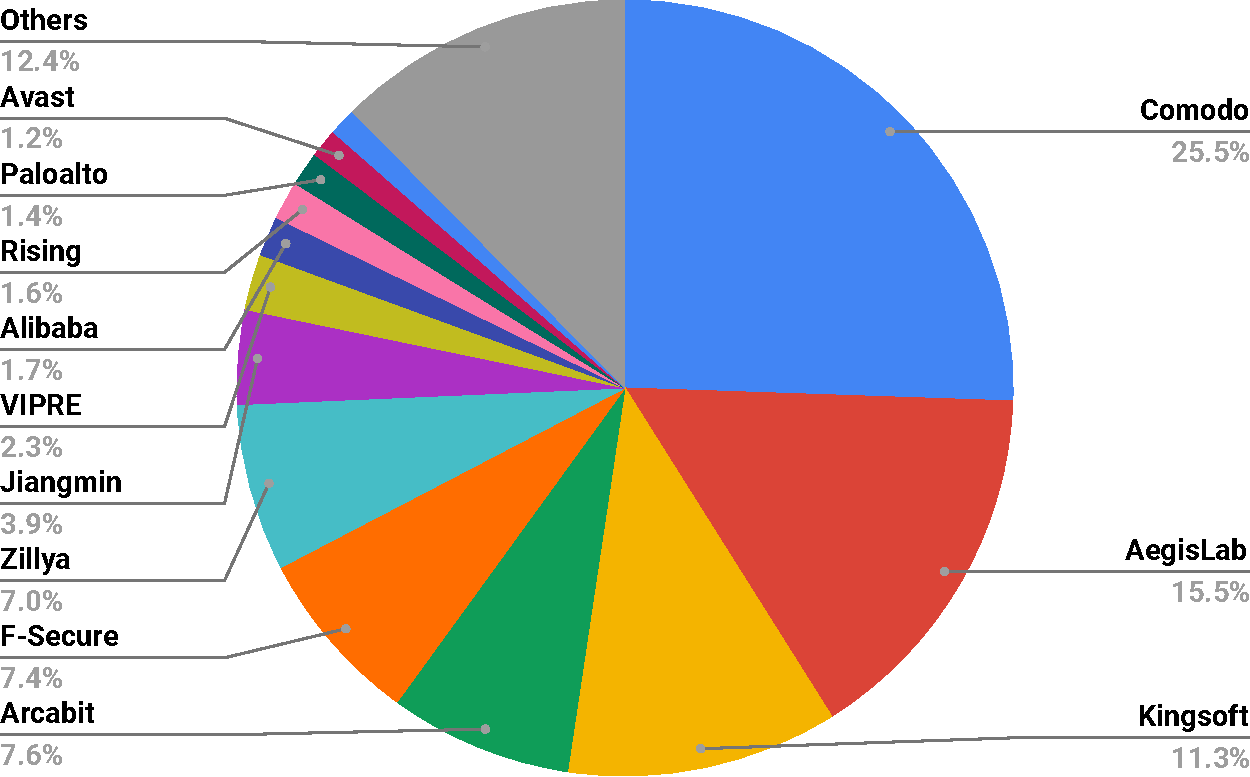
\includegraphics[width=\linewidth]{figure/hazard_vendorAll}
  \caption{Hazard distributions for vendors.
%(File types and their distributions for all VirusTotal submissions from 05/07/2016 to 09/06/2016.)
}
\label{fig:hazard_vendorAll}
  %\label{fig:overlap}
\endminipage\hfill
\minipage{0.31\textwidth}
  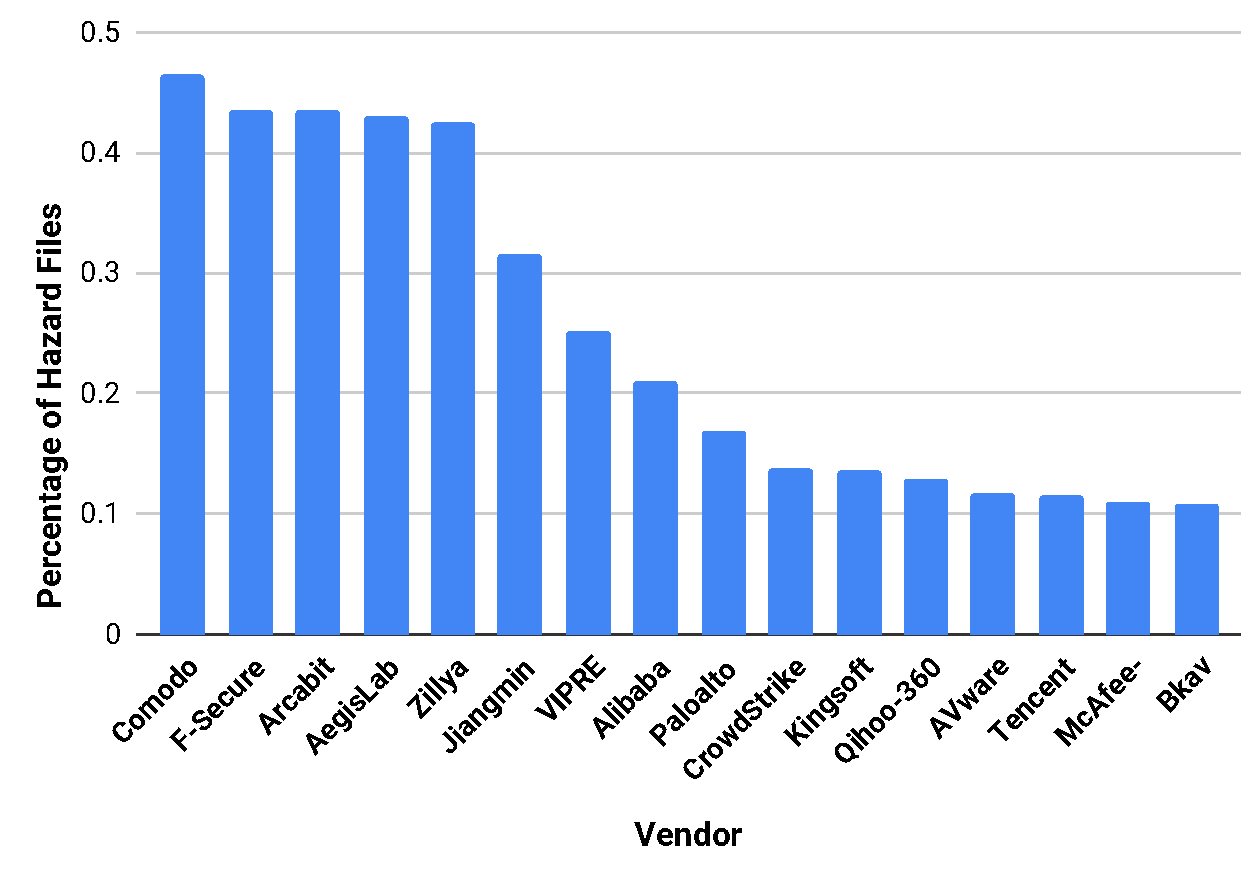
\includegraphics[width=\linewidth]{figure/hazard_vendorFile}
 \caption{Hazard file distributions for per vendor.
%{\footnotesize{
%(The number of suspicious files and the number of PE files submitted to VirusTotal from 05/07/2016 to 09/06/2016.)
%}
}
\label{fig:hazard_vendorFile}
  %\label{fig:maxUncover}
\endminipage\hfill
\minipage{0.31\textwidth}%
  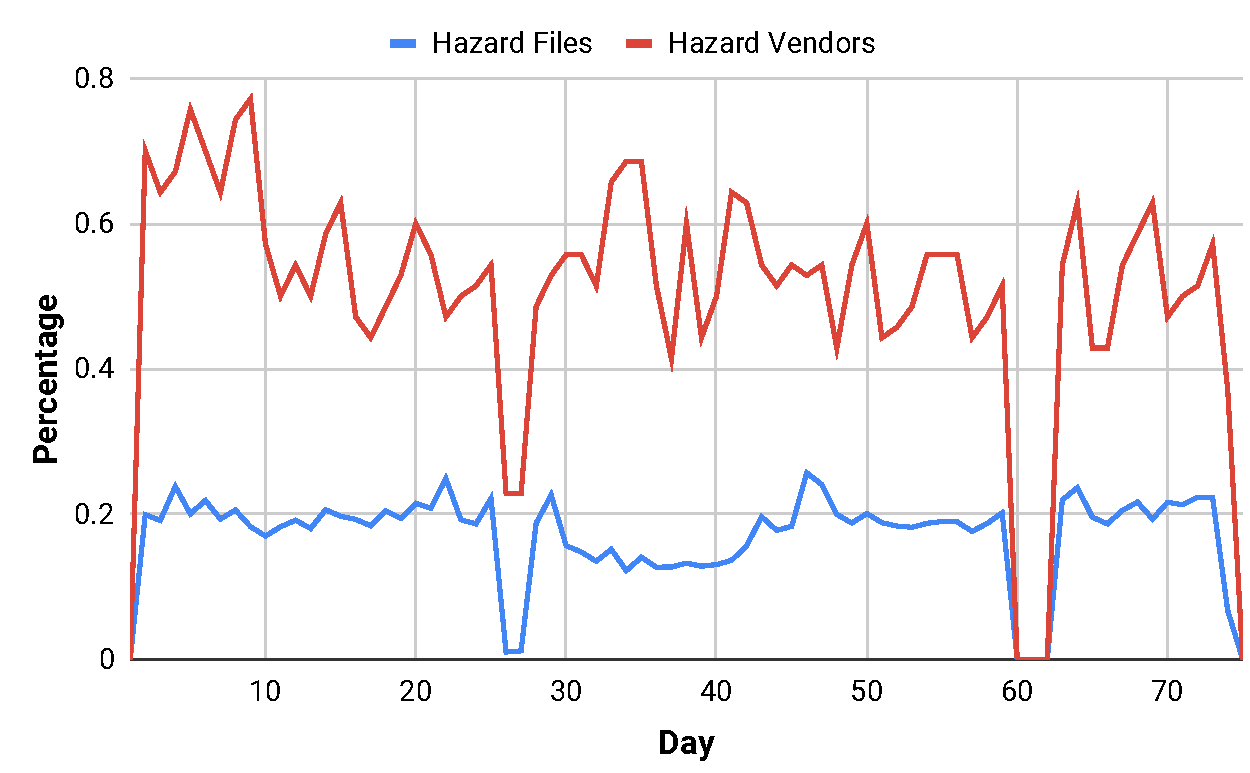
\includegraphics[width=\linewidth]{figure/hazard_day}
\caption{Hazard file and vendor distributions for per day.
%\footnotesize{
%(Only countries with more than 1\% PE submissions are shown.)
%}
}
\label{fig:hazard_day}
\endminipage\hfill

%\vspace{-0.2in}
\end{figure*}

Hazard pattern is an abnormal situation in the dection result sequences. It could affect the study of the other two patterns. So we first caculated the distribution of hazards over vendors, sampling files and days in our original data set.

In our statistics, only 3 vendors have no hazard patterns and other 67 vendors have hazards with different percentage. Hazards from the top 3 vendors accounts half of hazards and 13 vendors can cover more than 87\% hazards. Other 54 vendors have less than 1\% hazards, as shown in Figure \ref{fig:hazard_vendorAll}. Hazard pattern is quite frequently among vendors and sampling files.

Figure \ref{fig:hazard_vendorFile} shows the percentage of hazard files from top 16 vendors. Other vendors contains less than 10\% hazard files. "Comodo" contains the most hazards but has less than half of hazard files. We can make a conclusion from these results that hazard pattern is not caused by the engine misfunction. 

Figure \ref{fig:hazard_day} plots hazards distribution of files and vendors over every day. Overall, we find that hazard files randomly appear almost every day during these 75 days. The same conclusion can be made to hazard vendors. 

Figure \ref{fig:hazard_fileVendor} presents hazard file distribution over vendors. Only 4 hazard files involves more than 30 vendors and we did not find a file that its detection results from 70 vendors have hazard patterns. Thus, hazard pattern may not caused by the VirusTotal API.



%Todo: add hazard discussion in this part before discussing flipping. 

%Hazard caused by VT API? NO

%Hazard caused by vendor misfunction? NO

%conclusion: randomly appear, but quite frequently, affect lots of files

%Conclusion: remove hazard before studying flipping?

%Run experiments both with and without hazard
\textbf{Summary:} Hazard pattern is obviously common in our results and it affects lots of files and vendors. An immediate question that follows is what the results would be if we remove hazards before studying flipping and stable patterns? We will give more explanations of our experiments in the following sections.  

\subsection{Flipping Study}
%a. For each file, we count  of flipping vendors and  of flipping times

\begin{figure*}[!htb]
\minipage{0.31\textwidth}
  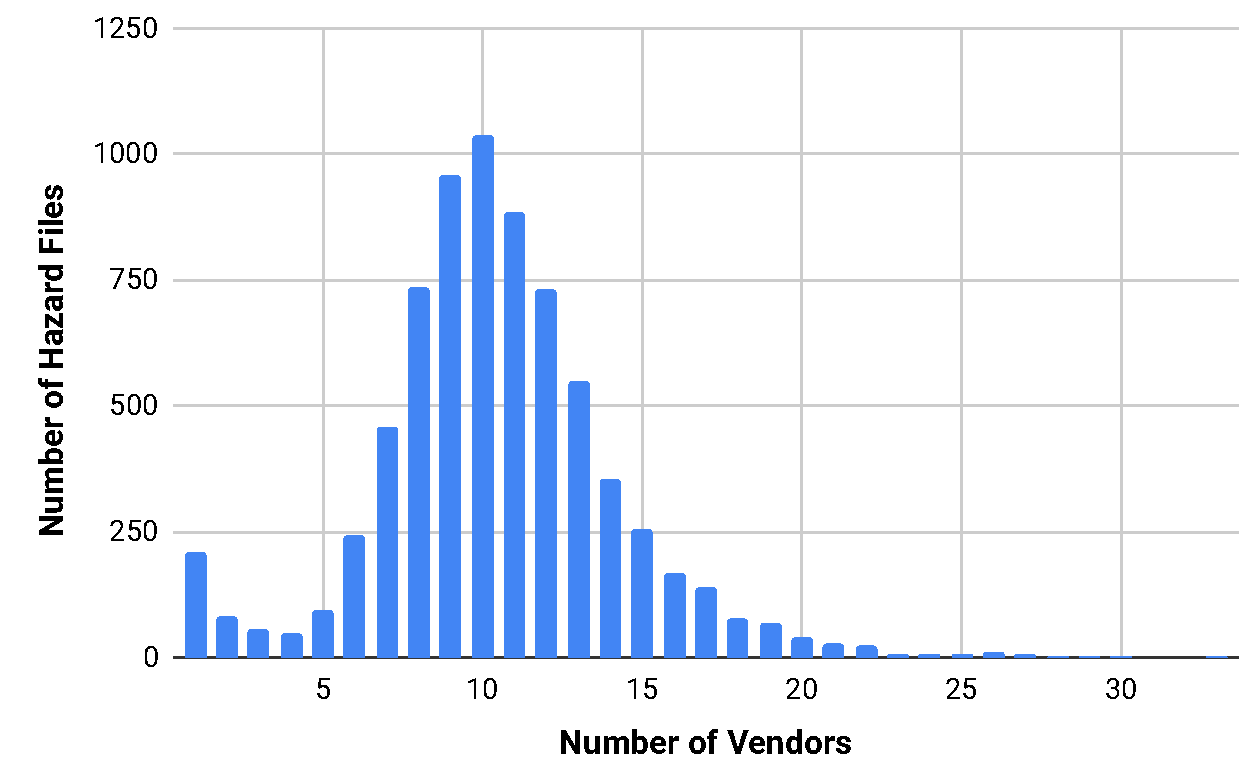
\includegraphics[width=\linewidth]{figure/hazard_fileVendor}
  \caption{Hazard file distributions over vendors.
%(File types and their distributions for all VirusTotal submissions from 05/07/2016 to 09/06/2016.)
}
\label{fig:hazard_fileVendor}
  %\label{fig:overlap}
\endminipage\hfill
\minipage{0.31\textwidth}
  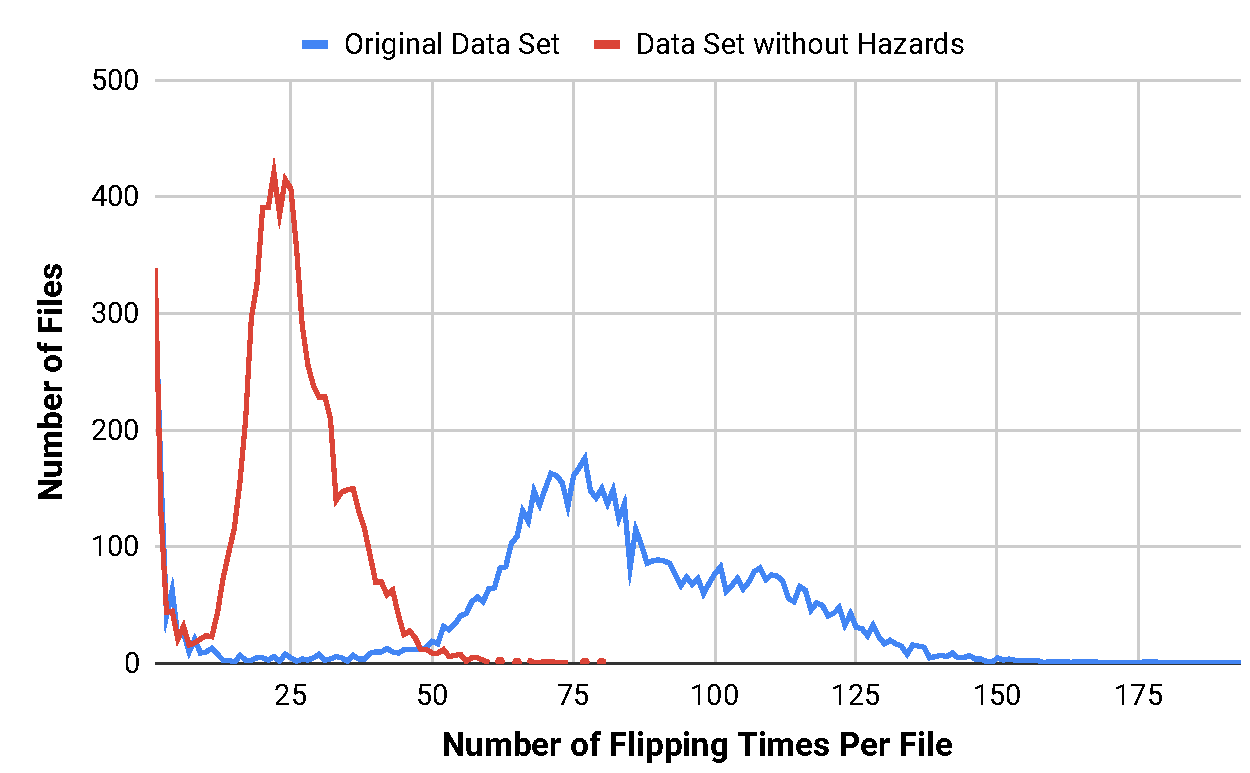
\includegraphics[width=\linewidth]{figure/flip_all}
 \caption{Flipping distributions for per file.
%{\footnotesize{
(The number of flipping times comparisons on data set both with and without hazards.)
%}
}
\label{fig:flip_all}
  %\label{fig:maxUncover}
\endminipage\hfill
\minipage{0.31\textwidth}%
  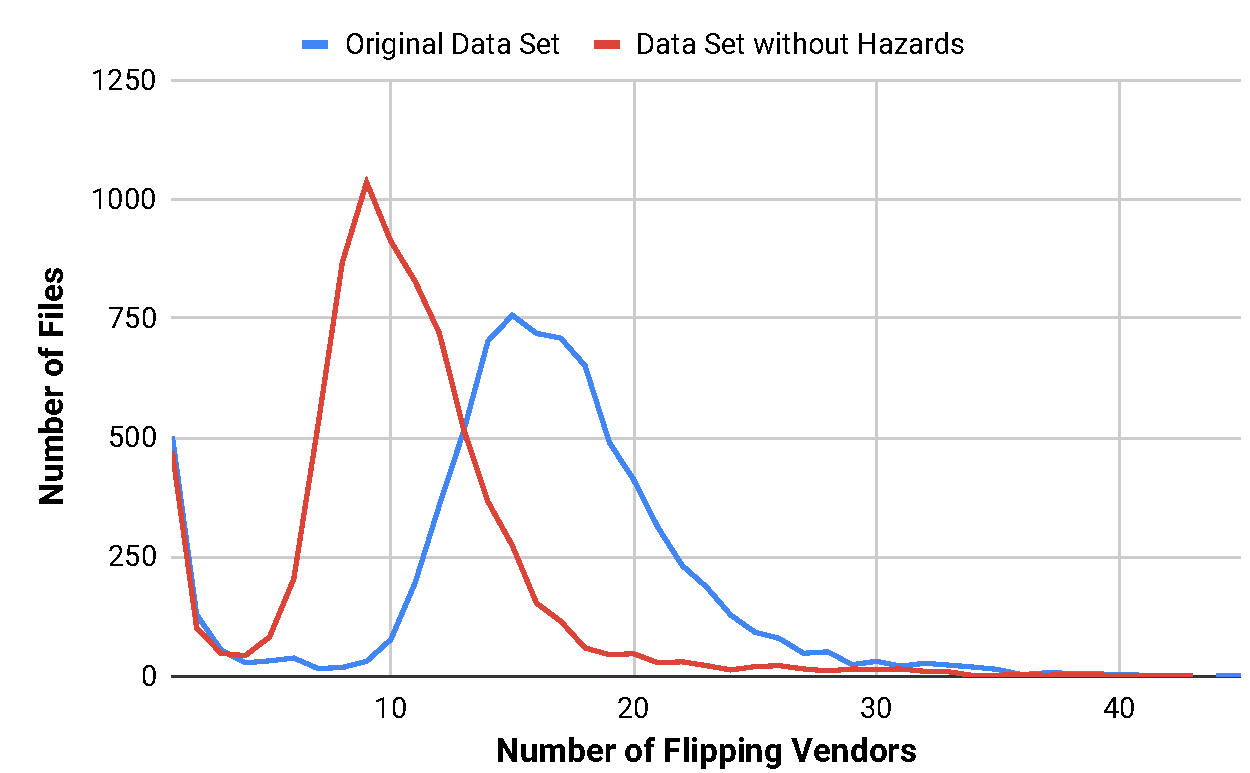
\includegraphics[width=\linewidth]{figure/flip_file}
\caption{Flipping vendor distributions for per file.
%\footnotesize{
(The number of flipping vendors comparisons on data set both with and without hazards.)
%}
}
\label{fig:flip_file}
\endminipage\hfill

%\vspace{-0.2in}
\end{figure*}

This section presents our results of flipping pattern study. As we discussed above, flipping pattern is an important pattern that affects a file to be stable. To study the flipping pattern, we calculate fippling distribution over files and vendors respectively in our original data set. Then, we remove hazards from our data set and recaulate the distributions for further comparison. 

Figure \ref{fig:flip_all} shows the distribution of flipping times for each file. Totally, we find that 7754 files have flipping patterns(total 14423), and the number drops to 7657 after smoothing hazards. Only 1 file have the largest flipping times of 193, and most files have only one flip. Without hazards, the largest flipping times is 80 and most files contian less flippings. For example, more than 421 files contain 22 flipping patterns. We can make the similar conclusion from the distribution of flipping vendors for each file, as shown in Figure \ref{fig:flip_file}. 

%b. For each vendor, we count  of flipping,  of flipping files, average flipping per file

To figure out the distribution of flipping pattern for each vendor, we calculate the flipping times, the number of flipping files from each vendor and the average flipping times per file. We run the same experiments both on our original data set and data set without hazards.

Overall, 68 vendors have flipping patterns(total 70), and "Comodo" contains more flipping patterns than other vendors. Some vendors, such as "Avast-Mobile" and "eGambit", have no flippings during the detction period. We present top 16 vendors ranking in the flipping list in Figure \ref{fig:flip_vendorAll}. Compared with results from the original data set, removing hazards has greatly reduced the flipping times for each vendor. 

Figure \ref{fig:flip_vendorFile} shows the distribution of flipping files for each vendor. 7 vendors have more than 40 percentage fippling files(total 14423). Removing hazards almostly does not affect the number of flipping files of some vendors. For some vendors, such as "Acrabit", "Zillya", "F-Secure", "CrowdStrike", we find the number of flipping files dramatically drops when we remove hazards from the original data set.

Figure \ref{fig:flip_vedorAvg} plots the average flipping times of a file from each vendor. We present 28 vendors that have more than 2 flipping times per file averagely, while other 42 vendors hold less than 2 flippings for each file. The most frequent flipping happens on "Comodo". On average, it contains more than 30 flipping times per file. Without hazards, the average flipping times significantly fall into almost half of original results. 

\begin{figure*}[!htb]
\minipage{0.31\textwidth}
  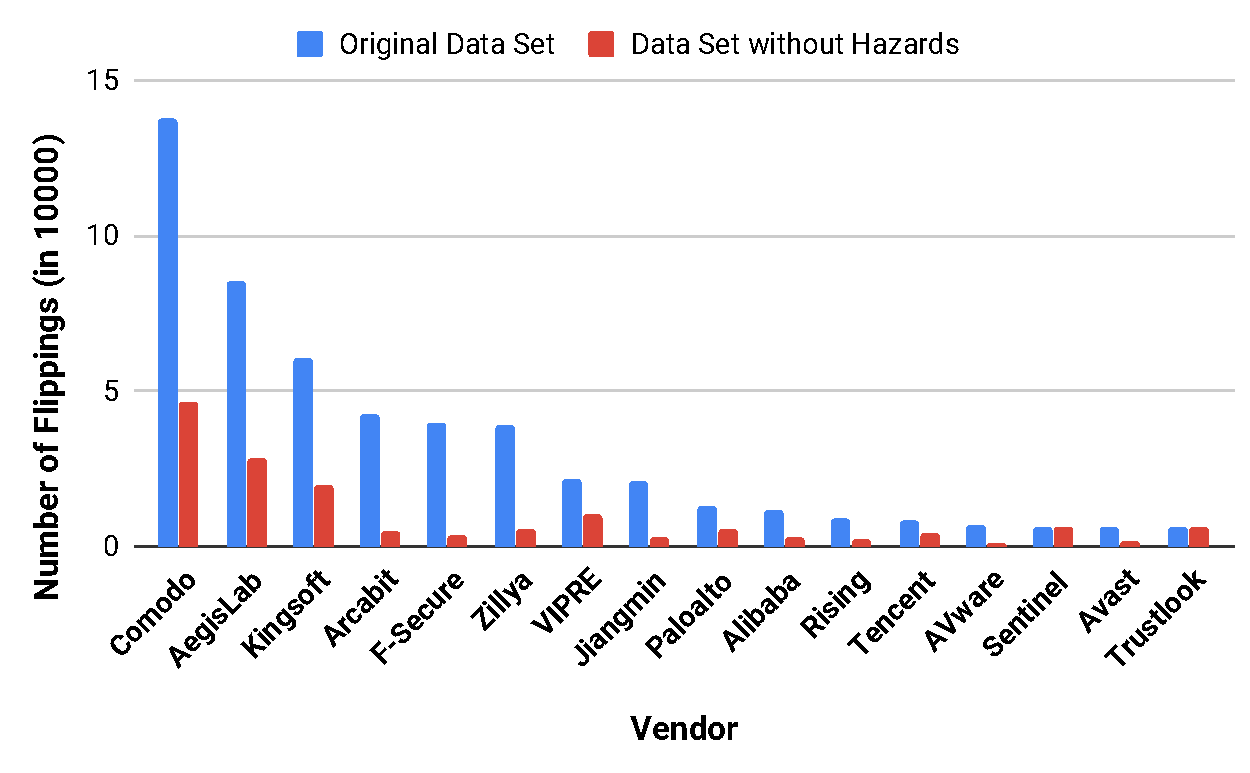
\includegraphics[width=\linewidth]{figure/flip_vendorAll}
  \caption{Flipping distributions for vendors.
(The number of flipping times for per vendor comparisons with and without hazards.)
}
\label{fig:flip_vendorAll}
  %\label{fig:overlap}
\endminipage\hfill
\minipage{0.31\textwidth}
  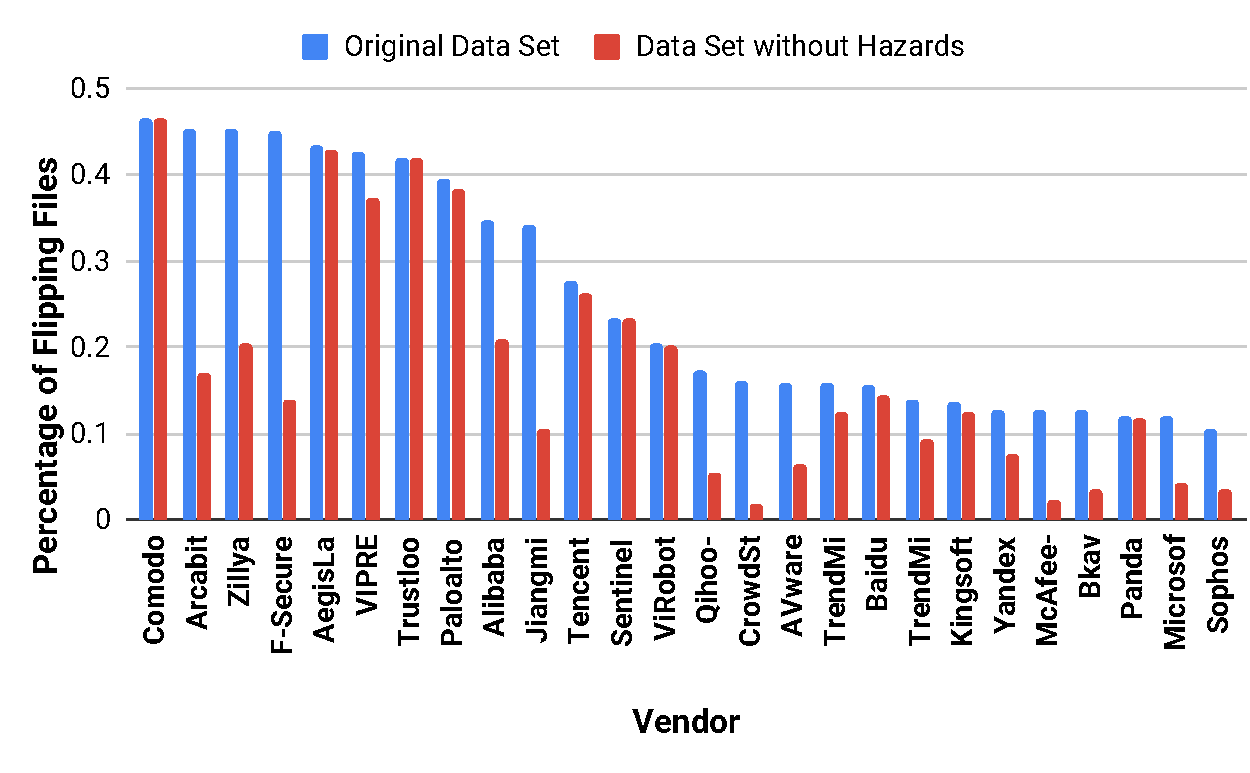
\includegraphics[width=\linewidth]{figure/flip_vendorFile}
 \caption{Flipping file distributions for per vendor.
%{\footnotesize{
(The number of flippings files for per vendor comparisons with and without hazards.)
%}
}
\label{fig:flip_vendorFile}
  %\label{fig:maxUncover}
\endminipage\hfill
\minipage{0.31\textwidth}%
  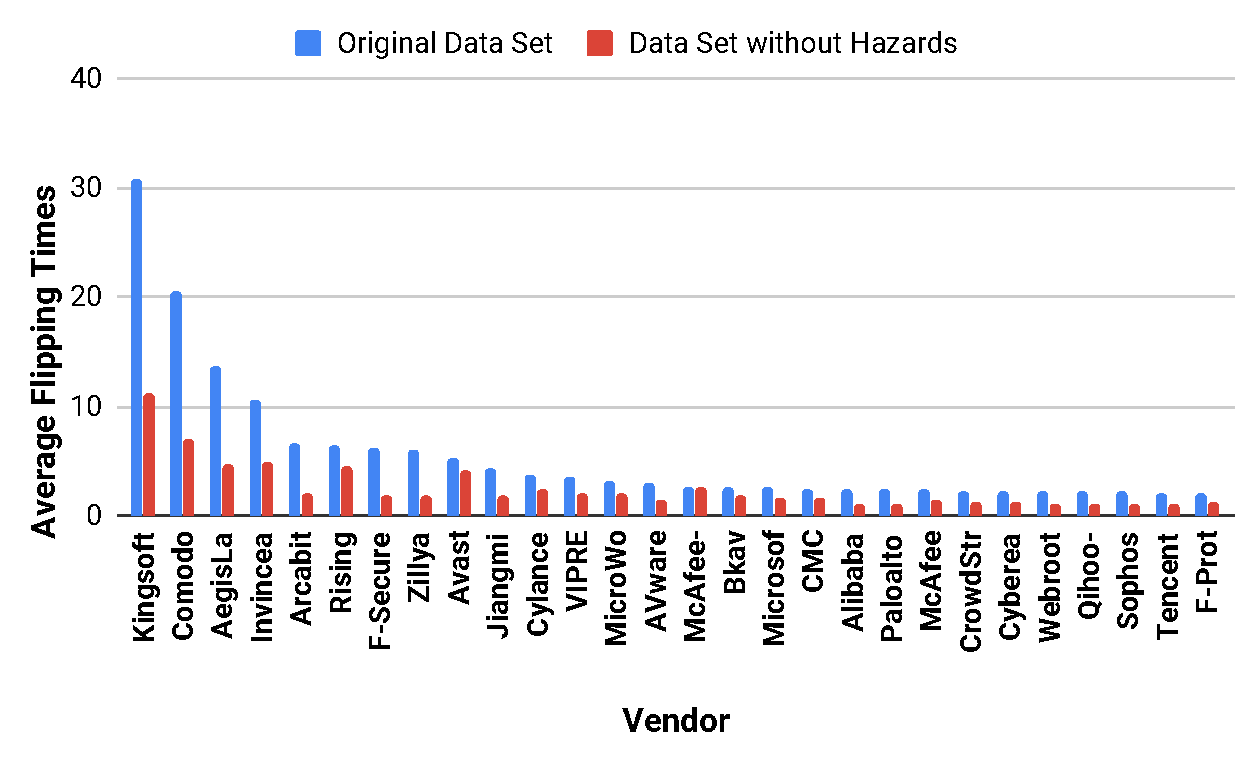
\includegraphics[width=\linewidth]{figure/flip_vendorAvg}
\caption{Average flipping times of a file for per vendor.
%\footnotesize{
(The average flipping times of a file for per vendor comparisons with and without hazards.)
%}
}
\label{fig:flip_vedorAvg}
\endminipage\hfill

%\vspace{-0.2in}
\end{figure*}

\textbf{Summary:} Flipping pattern widely exists in our experiments. Statistically, more than 50\% files and 97\% vendors have flipping patterns. Removing hazards is an effective approach to reduce flipping patterns for some vendors, but only 97 files have no flipping pattern after smoothing hazards. A large numbers of files and vendors still have flipping patterns. Flipping pattern is the most important reason that results in many files and vendors to be unstable.


\subsection{Stable Study}
a. We need some metrics to support our definition of ?stable? is reasonable.

b. Some metrics to show how long we need to wait until results become stable

\subsection{Conclusions}
